\section*{Глава 2. Реализация и тестирование}
\addcontentsline{toc}{section}{Глава 2. Реализация и тестирование}

\setcounter{section}{2}
\setcounter{subsection}{0}

\subsection{Реализация}
 Для реализации алгоритма DLT был использован MATLAB версии R2019b 9.7. Язык MATLAB - является высокоуровневым, имеет широкий спектр функций, интегрированную среду разработки, объектно-ориентированные возможности и интерфейсы к программам. Также, в нем имеются такие наборы инструментов, как Neural Network Toolbox и различные математические пакеты, удобные для вычисления сложных алгоритмов.
 
 \begin{figure}[h]
    \label{car4}
    \centering
    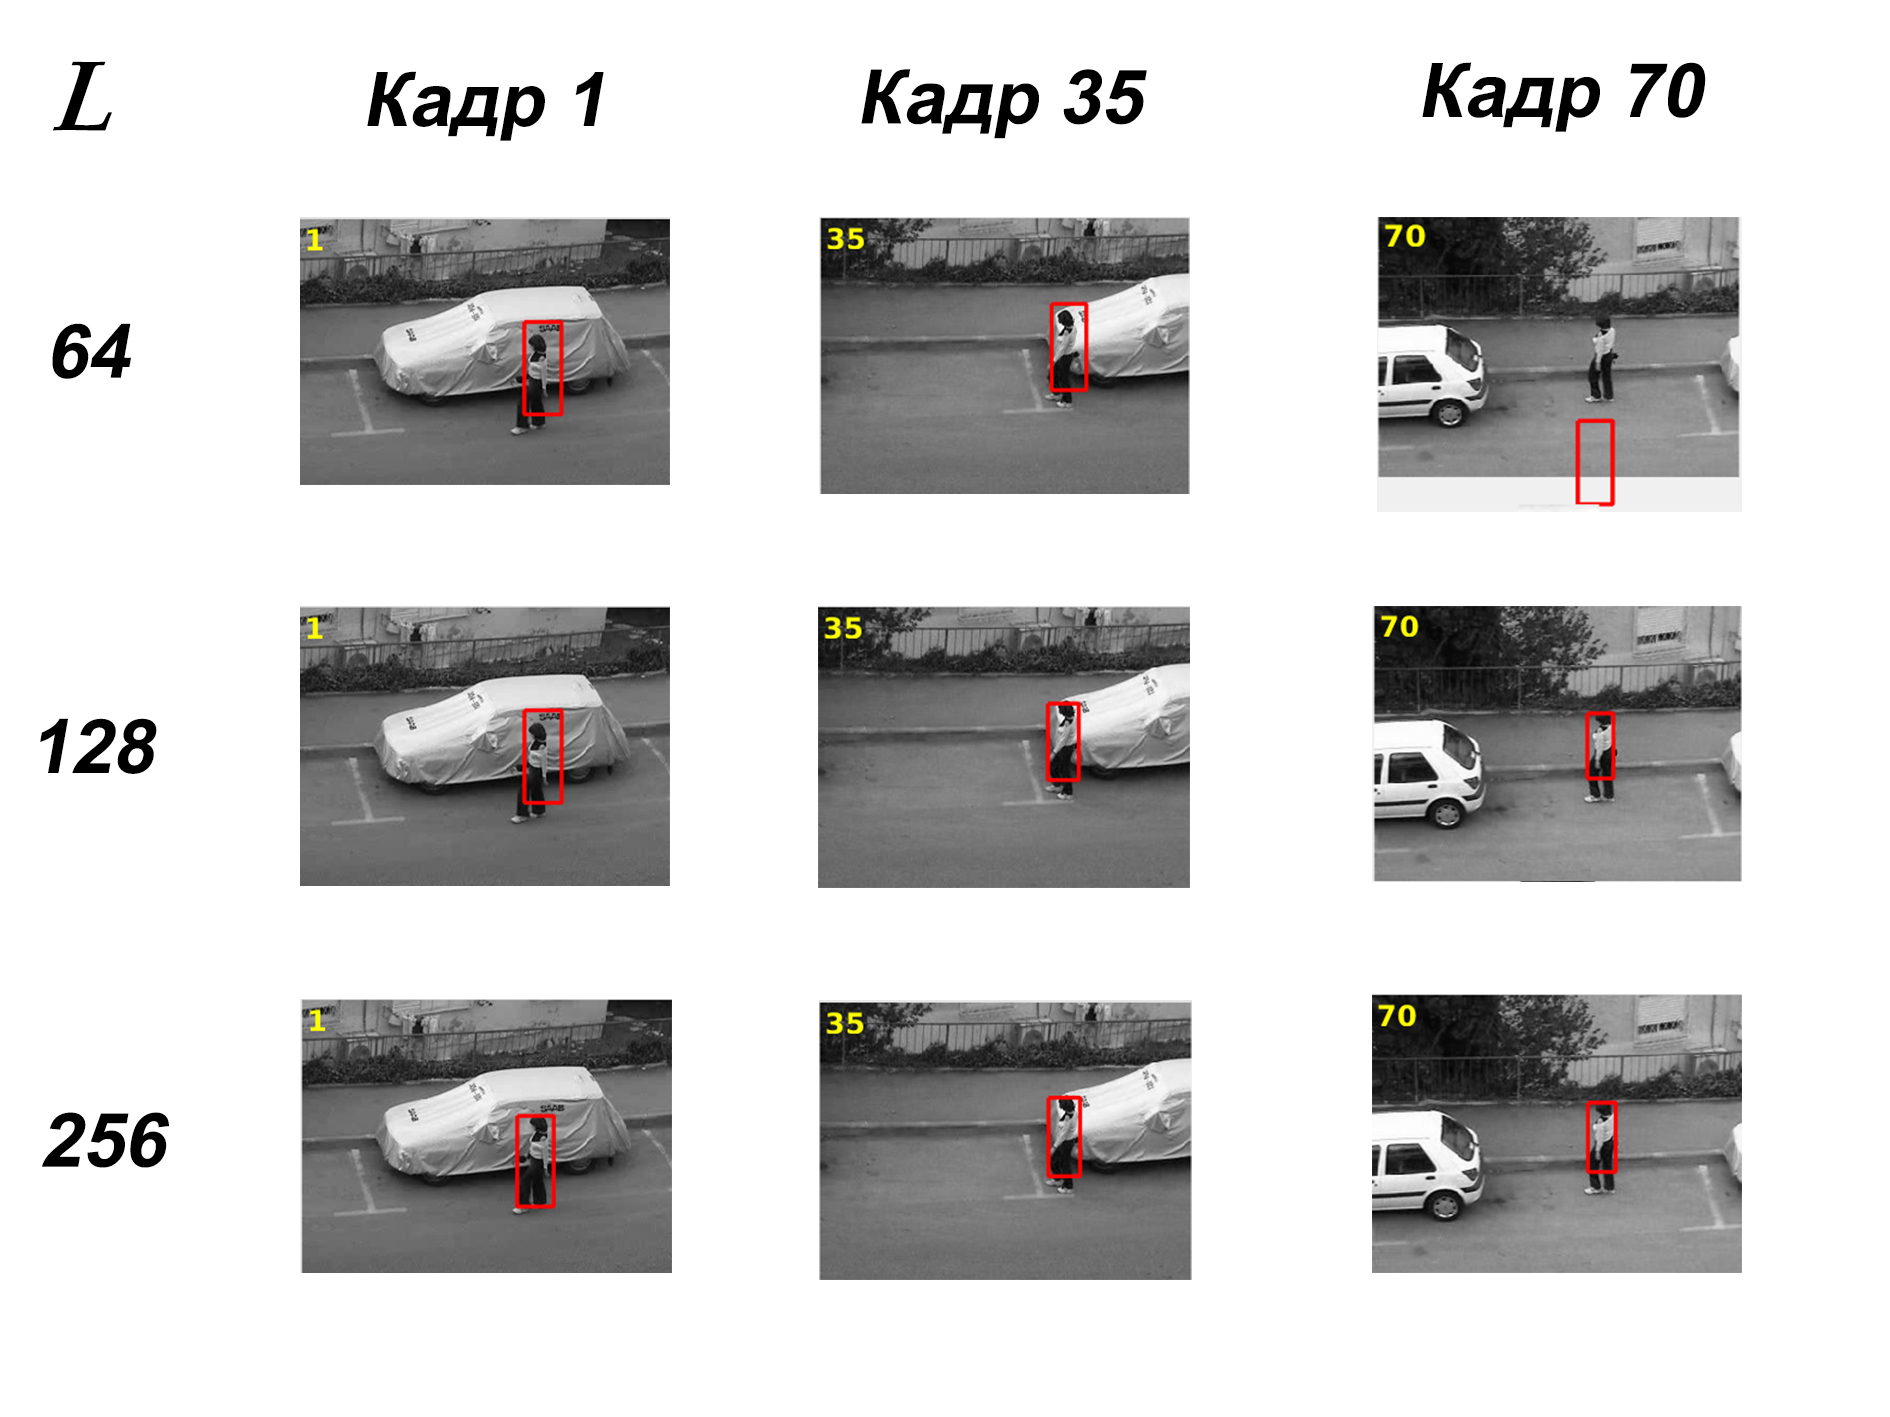
\includegraphics[width=10cm]{tests/img/Bez_imeni-2.jpg}
    \caption*{Рисунок 2.1 - Использование DLT на примере видео car4}
\end{figure}
 
 Также, можно наблюдать работу данной программы в режиме реального времени, наблюдая на экране по-кадровый вывод на котором красной рамкой демонстрируется траектория объекта, подсчитанная с помощью алгоритма DLT. На рисунке (2.1) мы можем наблюдать работу этой программы для конкретной последовательности car4.
 
 Для использования DLT необходимо изменить путь к папке с изображениями, которые мы хотим протестировать с помощью данного алгоритма в файле run\_individual.m и запустить его. На экране начнет появляться по-кадровая работа данного алгоритма. 
 
\subsection{Эксперименты}
\subsubsection{Входные данные}
В качестве входного набора изображений для тестирования оригинального и квантованного алгоритма, были использованы наборы изображений [4], разработанные специально для тестирования подобных моделей. В данной работе присутствует $50$ экземпляров видео, представленных в виде последовательности изображений, которые можно использовать для тестирования подобных программ слежения за объектами. 

В каждом наборе содержится последовательность кадров целостного видео в формате jpg или png, к которым прилагается файл. В данном файле присутствует таблица, содержащая в первом и втором столбце - координаты левого нижнего края объекта сначала по горизонтали, затем по вертикали соответственно; в третьем и четвертом - ширину и длину отслеживаемого объекта. С его помощью несложно определить точные координаты центра рамки и границ объекта для сравнения с полученными результатами.

За образцовый набор кадров были выбраны первые 70 кадров из последовательности Woman. Следует обратить внимание, что необходимо выбрать последовательность, которая будет хорошо работать на выбранном трекере. В силу того, что в экземплярах последовательностей, описанных ранее, в основном присутствуют образцы с определенными затруднениями, такие как: попадание объекта в тень или заходящим за какой либо объект, выходом за пределы кадра или со сложным фоном, специально для тестирования моделей в сложных ситуациях. Из всех данных видеоматериалов, был выбран стабильный участок последовательности, по причине исследования именно алгоритма квантования.

Тестирование проводилось с помощью процессора Intel(R) Pentium(R) CPU 2020M 2.40GHz. Заметим сразу, что вычисления можно ускорить, если вычисления проводить с помощью GPU и MATLAB Parallel Computing Toolbox, как для автономного обучения или квантования, так и для online-отслеживания.

\subsubsection{Реализация алгоритма квантования}

Необходимо выполнить квантование обученной матрицы весовых коэффициентов до начала работы онлайн обучения. Соответственно, для этого нужно выполнить алгоритм квантования весов и сохранить полученные результаты, для того чтобы в дальнейшем данные матрицы подгружались уже с квантованными весами. Также, следует квантовать веса с разным числом уровней квантования, для определения подходящего к данному трекеру числа и аналитике влияния этого числа на алгоритм.   

\begin{figure}[h!]
    \centering
    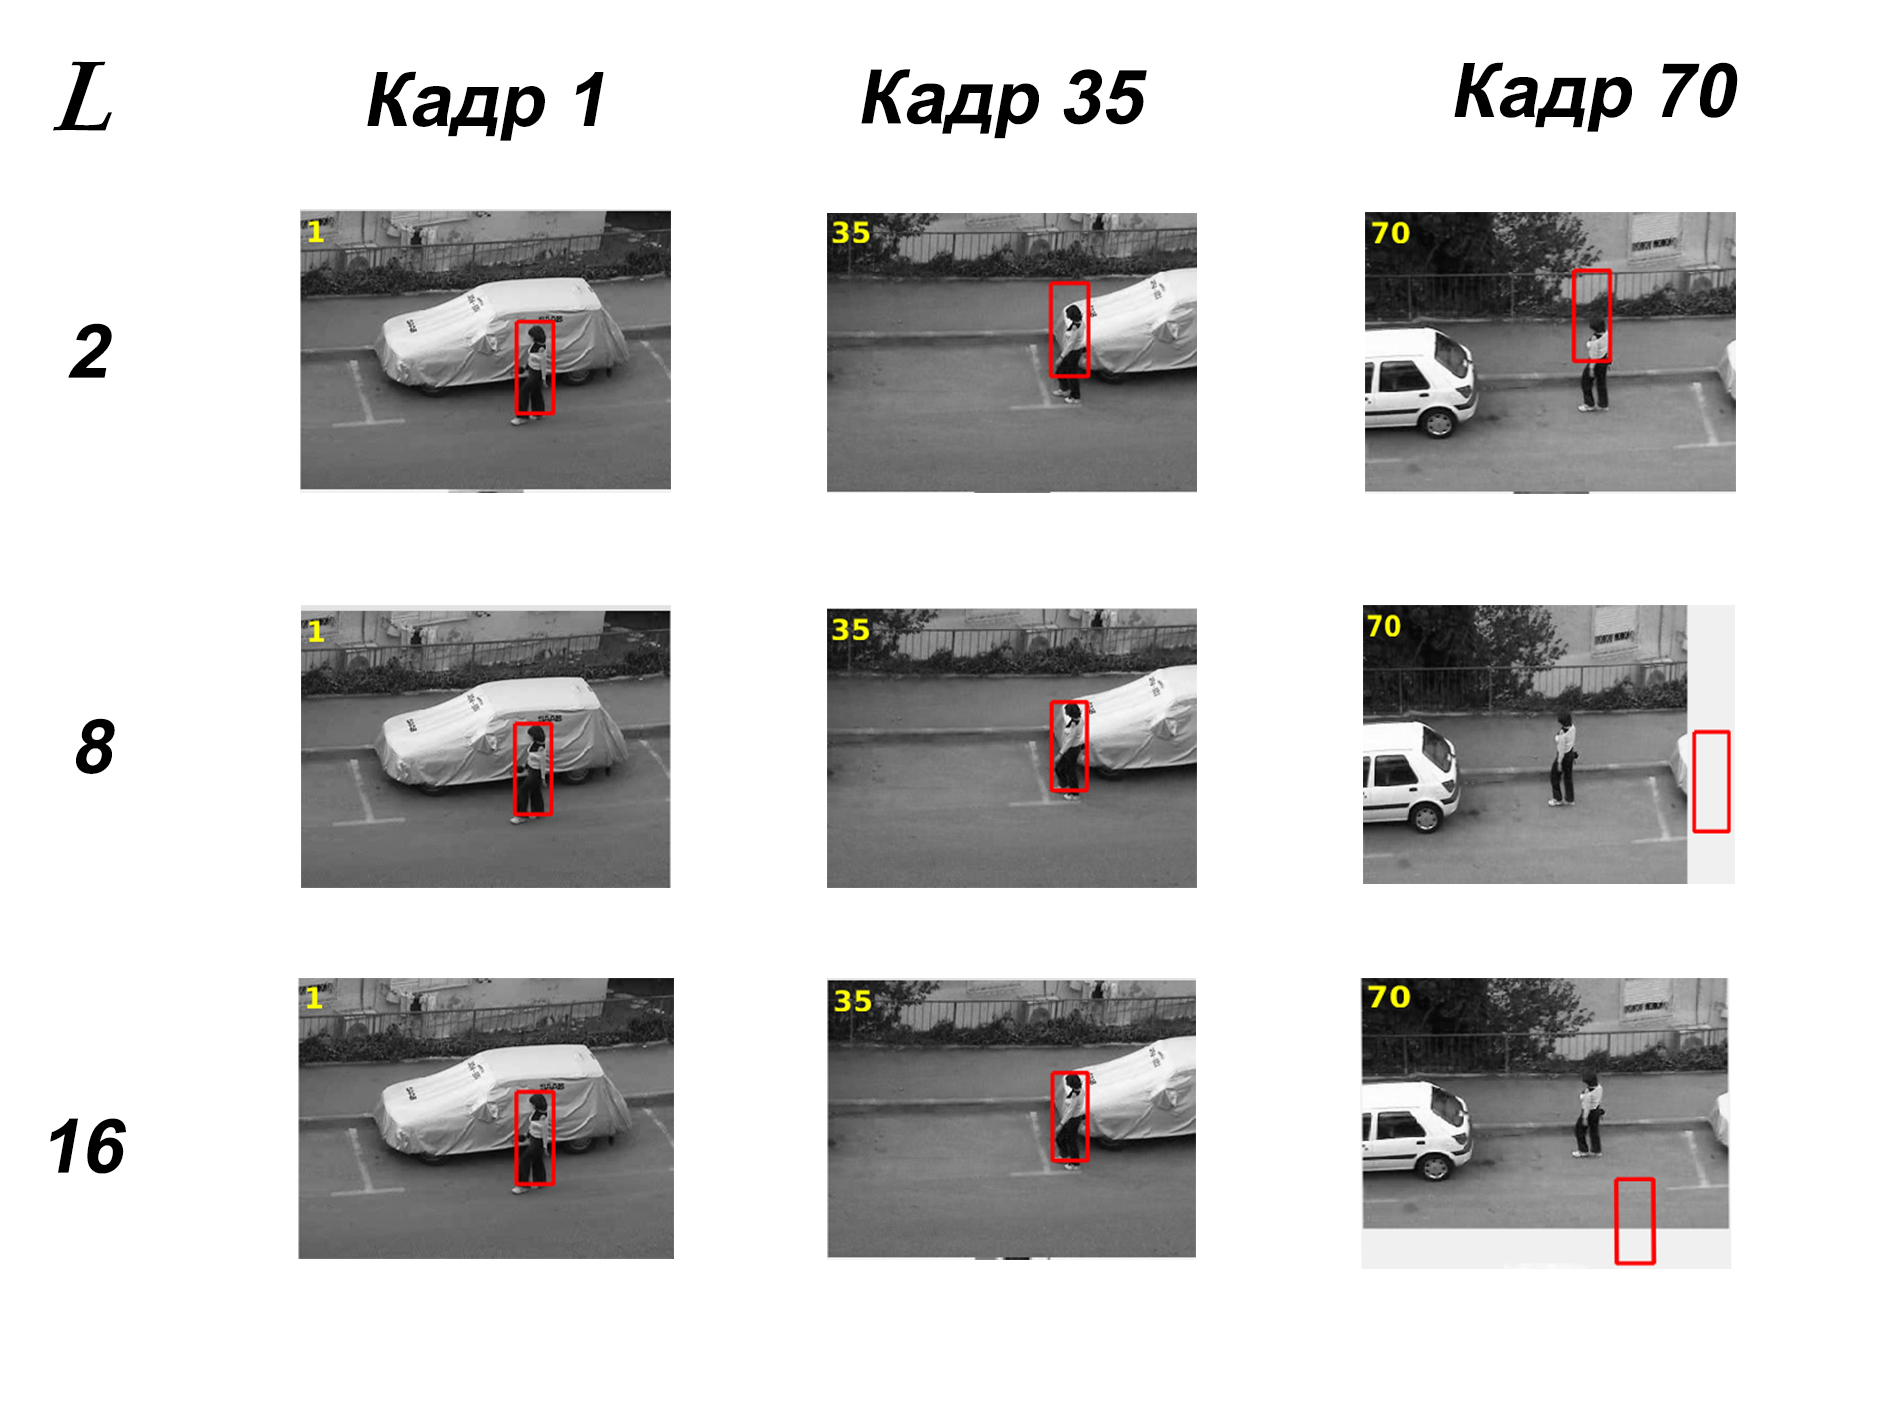
\includegraphics[width = 14 cm]{tests/img/Bez_imeni-1.jpg}
    \caption*{Рисунок 2.2 -- Работа алгоритма слежения. L - число уровней квантования}
\end{figure}

На основе вышеупомянутого, был реализован алгоритм квантования весовых коэффициентов сети (Приложение 1). Данный алгоритм запускается с разным значением параметра, отвечающего за число уровней квантования. Для определенности были выбраны следующие значения числа уровней квантования $L = 2,4,8,16,32,64,128,256$. В результате чего получаются наборы  данных, которые в последующем, вместо данного алгоритма, подгружаются на место весовой матрицы. Это необходимо для сокращения времени работы алгоритма и также для чистой оценки времени работы именно отслеживающего алгоритма.

\begin{table}[h!]
\caption*{Таблица 2.1 -- Значения памяти в зависимости от уровня квантования}
\begin{tabular}{|c|c|c|c|c|c|c|c|c|}
\hline
L                                                       & 2    & 4    & 8    & 16   & 32   & 64   & 128 & 256  \\ \hline
\begin{tabular}[c]{@{}c@{}}память\\ (в MB)\end{tabular} & 1.5 & 1.5 & 1.5 & 1.5 & 1.6 & 1.8 & 2.1  & 2.8\\ \hline
\end{tabular}
\end{table}

Память, занятая матрицами после выполнения алгоритма квантования, в зависимости от числа уровней квантования, представлена выше (Таблица -- 2.1). Заметим, что исходные весовые матрицы занимали 21MB, а получившиеся в результате квантования матрица, например при $L=128$ занимает 2.1 MB памяти, что в 10 раз лучше изначальных данных. 

\begin{figure}[h!]
    \centering
    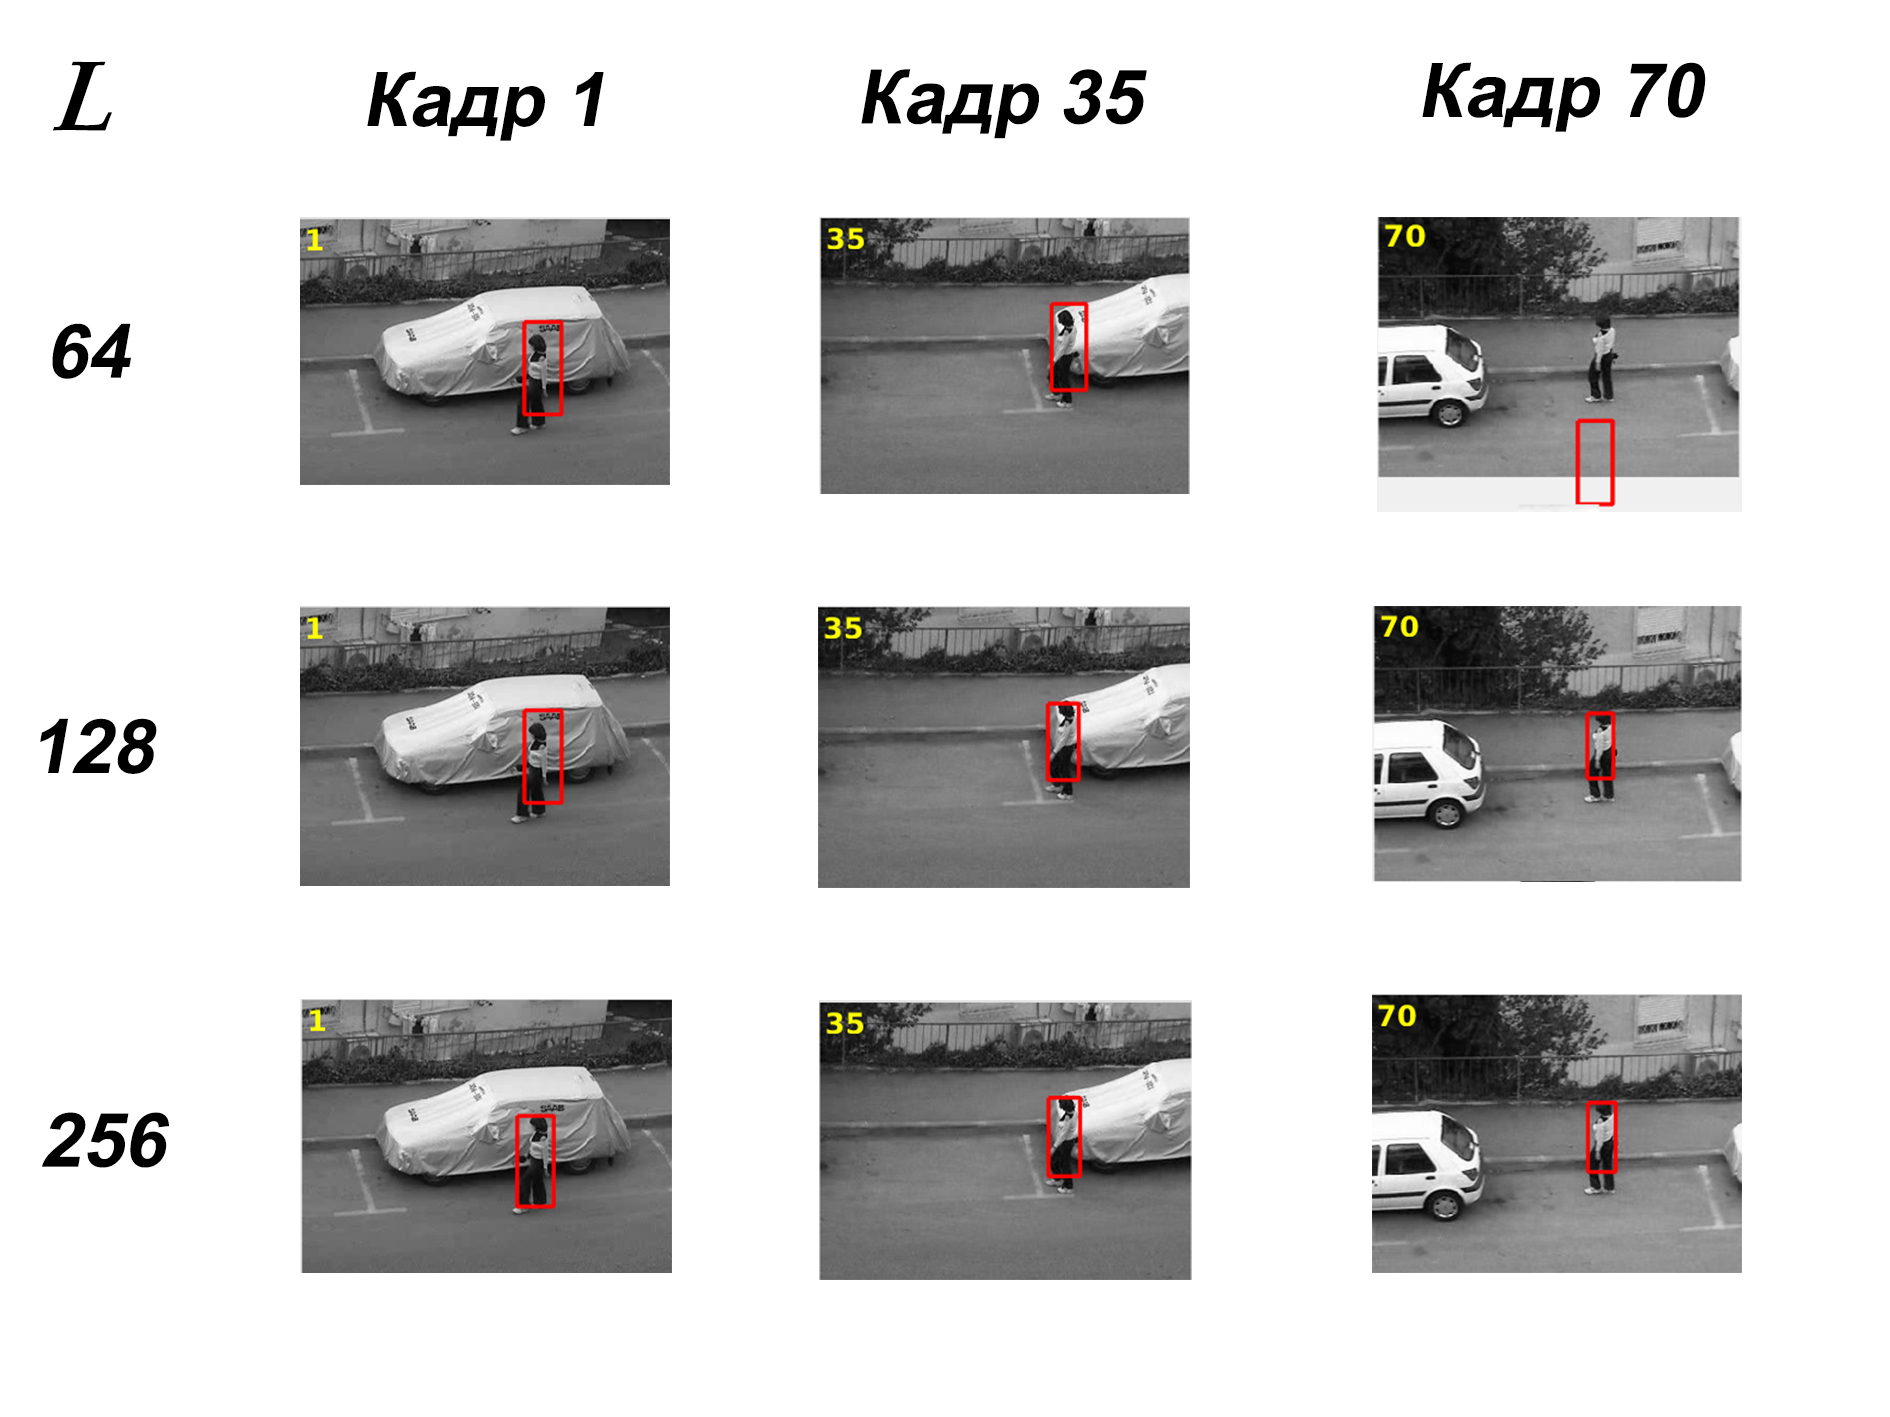
\includegraphics[width = 14 cm]{tests/img/Bez_imeni-2.jpg}
    \caption*{Рисунок 2.3 -- Работа алгоритма слежения. L - число уровней квантования}
\end{figure}

Таким образом, данный алгоритм запускается с разными квантованными матрицами, то есть матрицы с разным числом уровней квантования и на основе полученных результатов строится дальнейшая аналитика (Рисунок 2.2, 2.3). 

\subsubsection{Влияние квантования на время работы алгоритма}

Рассмотрим как меняется время работы алгоритма отслеживания с квантованными весовыми коэффициентами. Отметим, что время работы очень зависит от устройства, на котором запускается данная программа, и его параметров. В начале, мы зафиксируем время работы оригинального алгоритма слежения. Алгоритм DLT на выбранной последовательности без квантования весов работал в течение 47.51 секунд и с $fps = 1.47$ кадров в секунду. Далее, мы будем фиксировать три параметра для квантованного запуска программы - это общее время работы алгоритма отслеживания, количество кадров в секунду во время работы алгоритма и время, затраченное на квантование матриц.

Зависимость времени работы программы слежения от числа уровней квантования L представлена ниже (Таблица 2.2). По данной таблице мы можем наблюдать уменьшение времени работы алгоритма отслеживания от числа уровней квантования. 

\begin{table}[h!]
\caption*{Таблица 2.2 -- Зависимость времени от числа уровней квантования}
\begin{tabular}{|c|c|c|c|}
\hline
L   & \begin{tabular}[c]{@{}c@{}}Время работы\\  программы\end{tabular} & \begin{tabular}[c]{@{}c@{}}Количество кадров\\  в секунду (fps)\end{tabular} & \begin{tabular}[c]{@{}c@{}}Время квантования\\   матриц\end{tabular} \\ \hline
2   & 75.4                                                              & 0.93                                                                         & 10.2                                                                 \\ \hline
4   & 73.8                                                              & 0.95                                                                         & 10.1                                                                 \\ \hline
8   & 74.6                                                              & 0.94                                                                         & 12.3                                                                 \\ \hline
16  & 72.6                                                              & 0.96                                                                         & 18.6                                                                 \\ \hline
32  & 72.6                                                              & 0.96                                                                         & 30.1                                                                 \\ \hline
64  & 74.6                                                              & 0.94                                                                         & 54                                                                   \\ \hline
128 & 45.7                                                              & 1.53                                                                         & 105.3                                                                \\ \hline
256 & 43.9                                                              & 1.6                                                                          & 202                                                                  \\ \hline                     
\end{tabular}
\end{table}

При $L = 2,4,..,64$ значительных изменений во времени не наблюдается. Худший результат наблюдается при $L=2$. Во время работы алгоритма при таких значениях уровня квантования наблюдается слишком частое подобучение, то есть происходит онлайн обучение сети на конкретном кадре, в следствие чего время работы по сравнению с непрерывными весами увеличивается. При $L = 128$ и $L = 256$ время алгоритма схоже с оригинальным значением времени.

Количество кадров в секунду берется в среднем за все время работы алгоритма. Наблюдается уменьшение данного показателя при подобучении, увеличение при его отсутствии, и, также, как и параметр общего времени, с увеличением числа уровней квантования количество кадров в секунду растает.

Время квантования матриц, начиная от $L=8$ растет линейно, относительно числа уровней квантования. Другими словами, время квантования увеличивается примерно в 2 раза при увеличении числа уровней квантования в 2 раза. Это наблюдается в силу одного вхождения цикла по L в реализацию алгоритма квантования. 

Для большей наглядности, для полученных данных была реализована диаграмма (Рисунок 2.4). С ее помощью можно наблюдать динамику изменения времени относительно числа уровней квантования и сравнение с изначальным значением времени. 

\begin{figure}[h!]
    \centering
    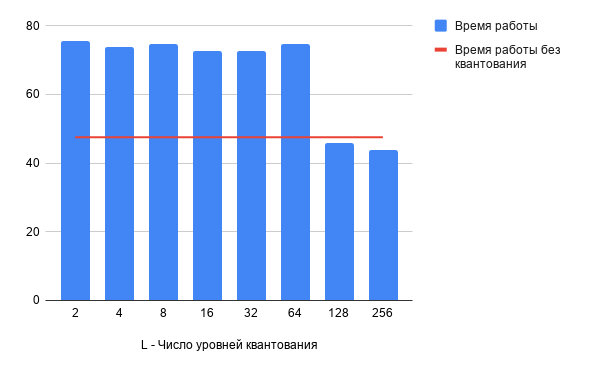
\includegraphics[width = 14 cm]{tests/img/time.png}
    \caption*{Рисунок 2.4 -- Зависимость времени от числа уровней квантования }
    \label{fig:my_label}
\end{figure}

Таким образом, из данного рассуждения следует, что лучшие результаты достигнуты с точки зрения времени при $L = 128, 256$, наихудшие -- при $L=2$.

\subsubsection{Влияние квантования на смещение центра}

Для определения смещения центра объекта алгоритмом, необходимо снять координаты перемещения для него с неквантованными весовыми коэффициентами. Сначала, вычисляются координаты смещения для исходного алгоритма DLT. Далее, снимаются аналогичные координаты, но уже после квантования весов для различных уровней квантования, и определяется модуль разницы между исходным алгоритмом и модифицированным. Таким образом, получается смещение, которое может показывать качество работы алгоритма слежения за объектами.

\begin{figure}[h!]
    \centering
    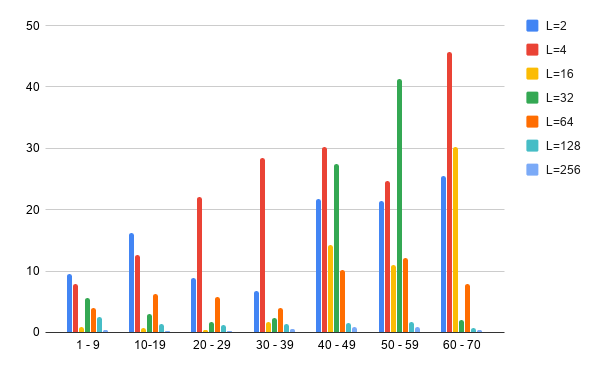
\includegraphics[width = 14 cm]{tests/img/diag_x.png}
    \caption*{Рисунок 2.5 -- Смещение центра по горизонтали от числа уровней квантования}
    \label{fig:my_label}
\end{figure}

В результате данной работы были определены смещения центра объекта для следующих чисел уровней квантования $L = 2, 4, 16, 32, 128, 256$. Работая с координатами центра рамки, все вычисления разделяются  на значения по горизонтали и вертикали. Полученные данные были занесены в таблицы сначала относительно горизонтальной координаты (Приложение 2).

Также, выше представлен рисунок, полученный на основе данной таблицы, для более наглядного представления относительно большого объема данных (Рисунок 2.5).

\begin{figure}[h!]
    \centering
    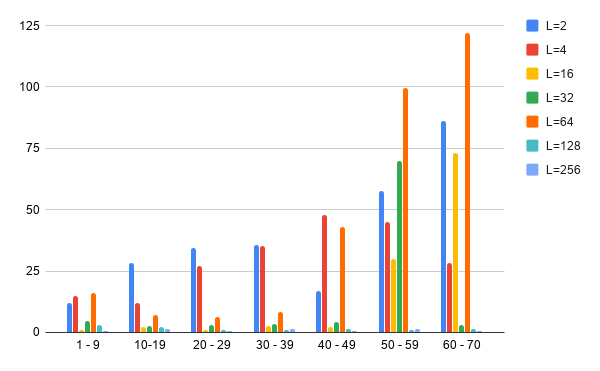
\includegraphics[width = 13 cm]{tests/img/diag_y.png}
    \caption*{Рисунок 2.6 -- Смещение центра по вертикали от уровней квантования}
    \label{fig:my_label}
\end{figure}

Такие подробные данные позволяют покадрово определить в каких именно изображениях ухудшается слежение. Так, например, можно заметить сильное смещение в последних кадрах последовательности при $L=4$.

Полученные рассуждения можно повторить и для вычисления смещения центра рамки по вертикали (Приложение 3) и аналогично рассмотреть полученные результаты на рисунке (Рисунок 2.6). По данному рисунку видно, что также как и по горизонтали, здесь наблюдается усиление смещения к концу последовательности. 

\begin{table}[h!]
\caption*{Таблица 2.3 -- Зависимость смещения центра от числа уровней квантования}
\begin{tabular}{|c|c|c|}
\hline
\multirow{2}{*}{L} & \multicolumn{2}{c|}{\begin{tabular}[c]{@{}c@{}}Среднее смещение\end{tabular}}                                                                      \\ \cline{2-3} 
                   & \begin{tabular}[c]{@{}c@{}}по горизонтали (по координате x)\end{tabular} & \begin{tabular}[c]{@{}c@{}}по вертикали (по координате y)\end{tabular} \\ \hline
2                             & 16,2                                   & 41,9                                 \\ \hline
4                             & 24,4                                   & 30,2                                 \\ \hline
8                             & 41                                     & 7,6                                  \\ \hline
16                            & 8,4                                    & 17                                   \\ \hline
32                            & 11,8                                   & 13                                   \\ \hline
64                            & 7,2                                    & 44,7                                 \\ \hline
128                           & 1,6                                    & 1,6                                  \\ \hline
256                           & 0,5                                    & 0,9                                  \\ \hline
\end{tabular}
\end{table}

По данным относительно каждого кадра исследуемой последовательности, необходимо сделать усреднение, чтобы определить качество работы данного алгоритма для каждого уровня квантования в среднем. Полученные данные занесены в таблицу зависимости среднего смещения центра рамки захвата (в пикселях) от числа уровней квантования (Таблица 2.3).

Из полученных данных наблюдается уменьшение ошибки с увеличением числа уровней квантования, после значения $L=64$. При $L = 128$  b $L=256$ для смещений происходит существенное уменьшение данного параметра. Таким образом, можно выбрать какое смещение будет наиболее приемлемо. Наихудшее среднее смещение наблюдается как при $L=2$, так и при $L=64$, а при $L=256$ -- наилучшее. При этом, можно отметить, что значения при $L=128$  вполне приемлемы, хотя временные затраты на реализацию и объем памяти меньше, чем у лучшего кандидата.     

\begin{figure}[h!]
    \centering
    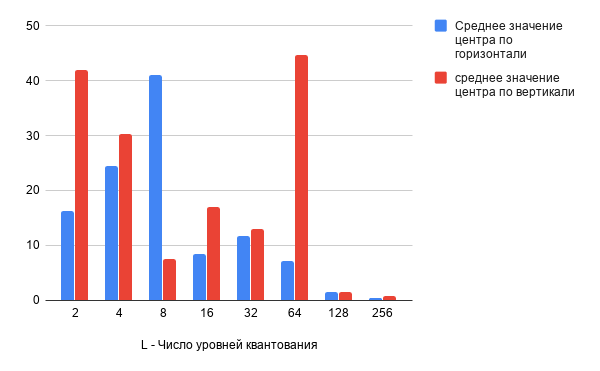
\includegraphics[width = 14 cm]{tests/img/sm.png}
    \caption*{Рисунок 2.7 -- Зависимость смещения центра от числа уровней квантования}
\end{figure}

Далее, проиллюстрируем таблицу, упомянутую выше, с помощью столбчатой диаграммы, изображенной на рисунке (Рисунок 2.7). На ней заметна разница между средним смещением центра рамки по вертикали и по горизонтали. 

По полученным данным смещения и среднего смещения центра отслеживающей рамки отчетливо видны слишком большие изменения (как в последних кадрах) и незначительные, близкие к исходному (как при $L=128,256$). В дополнении к этому, хотелось бы проанализировать для каждого кадра, теряет ли трекер отслеживаемый объект. Другими словами, насколько значительно 
полученное смещение для отслеживания выбранного объекта. Данный анализ можно произвести зрительно, с помощью выводимых кадров во время работы программы, но данный способ не надежен и имеет субъективный характер.

Для получения желаемых результатов, вычисляется относительное смещение в зависимости от числа уровней квантования. Для вычисления данных параметров необходимо полученные выше смещения центра рамки относительно каждого кадра разделить (в случае горизонтальной координаты) на ширину соответствующего кадра последовательности. Полученные результаты представлены в виде таблицы (Приложение 4). Из данной таблицы следует, что вплоть до $L=64$, отслеживание объекта по горизонтали происходит с потерей объекта, при $L=128$ -- ни в одном кадре не теряется объект, а при $L=256$ -- остается достаточно мало кадров, в которых смещение отлично от нуля. 

\begin{figure}[h!]
    \centering
    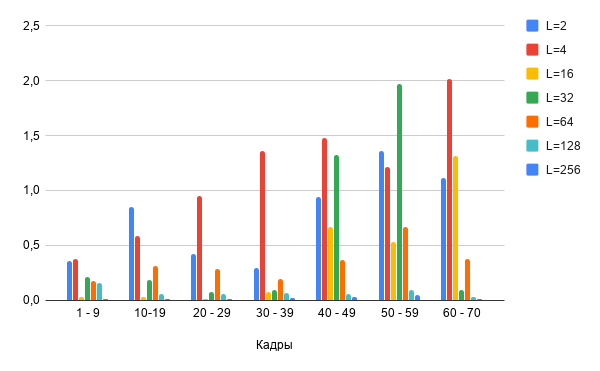
\includegraphics[width = 14 cm]{tests/img/diag_rlt_disp_x.png}
    \caption*{Рисунок 2.8 -- Относительное смещение (горизонталь) от уровней квантования}
\end{figure}

По полученной таблице была реализована диаграмма, изображенная на рисунке (Рисунок 2.8). Аналогичные рассуждения можно провести и для смещений центра рамки по вертикали, в данном случае разделив соответствующие смешения на соответствующую длину (Приложение 5). 

\begin{figure}[h!]
    \centering
    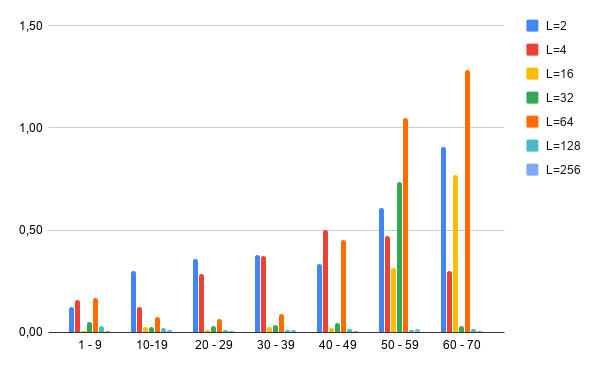
\includegraphics[width = 14 cm]{tests/img/diag_rlt_disp_y.png}
    \caption*{Рисунок 2.9 -- Относительное смещение (вертикаль) от уровней квантования}
\end{figure}

На иллюстрации вертикального относительного смещения (Рисунок 2.9), в отличие от горизонтального, наблюдается иные результаты. При $L = 2,4,..,64$ показатели превышают 1, что свидетельствует о потери объекта алгоритмом отслеживания. Но не смотря на это, при $L = 128,256$ ни в одном кадре не теряется объект.

В результате данных экспериментов, можно сделать вывод о числе уровней квантования, достаточном для
качественного отслеживания положения объекта в кадре. При $L = 128, 256$ наблюдается хорошее качество отслеживания. В зависимости от желаемой точности, времени и занимаемой памяти, выбираемые уровни обеспечивают надежность отслеживающего алгоритма.
